\documentclass{article}

% Sim2Science @ NeurIPS 2026 -- per the CFP, the workshop track of the official
% NeurIPS 2026 style, double-blind. 5 pages excluding references; the
% reproducibility checklist goes after the references and does not count.
\usepackage[dblblindworkshop]{neurips_2026}
\workshoptitle{Sim2Science}

\usepackage[utf8]{inputenc}
\usepackage[T1]{fontenc}
\usepackage{hyperref}
\usepackage{url}
\usepackage{booktabs}
\usepackage{amsfonts}
\usepackage{nicefrac}
\usepackage{microtype}
\usepackage{graphicx}
\usepackage{subcaption}

\newcommand{\ming}[1]{\textcolor{red}{#1}}
\graphicspath{{figures/}}

% z_phys / z_inst appear constantly; one macro each keeps them consistent
\newcommand{\zphys}{z_{\mathrm{phys}}}
\newcommand{\zinst}{z_{\mathrm{inst}}}

\title{Causal model for disentangling time-series representation in Gaia and ZTF surveys}

\author{%
  Anonymous Author(s) \\
  Affiliation \\
  Address \\
  \texttt{email} \\
}

\begin{document}

\maketitle

\begin{abstract}
TODO.
\end{abstract}

\section{Introduction}
TODO.

\section{Method}

\paragraph{Dataset preparation.}
The sample is assembled in five steps, each of which leaves a footprint the later analysis has to know about:
\begin{itemize}\itemsep0pt
\item \emph{Labels and matching.} Variable-star classes come from the VSX catalogue. ZTF lightcurves are matched to VSX positions, and VSX stars to Gaia DR3 epoch photometry by positional matching at $1.5''$, which retains 74.8\% of the VSX stars.
\item \emph{A transitive join.} ZTF and Gaia are therefore joined through the VSX position rather than directly. The two catalogues sit at different epochs (J2000 against J2016.0), so proper motion could break a match and would show up as a separation growing with parallax; the separation is flat across parallax bins (Spearman $-0.09$). One consequence is that the sample contains only low-proper-motion stars and no transients.
\item \emph{Epoch floors.} At least 8 usable ZTF epochs, leaving 109,598 stars. The matching Gaia floor is inert, since three transits already unroll to nine $G$/$BP$/$RP$ rows, so the floor is entirely a ZTF cut.
\item \emph{Taxonomy.} Dropping the VAR and MISC families and capping each class at 8,000 gives the final 34,386 stars in 8 classes (E, EC, ELL, L, M, RRAB, SR, SRS). The Gaia match is label-correlated (pulsators are retained more often than eclipsers), so this class mix is not the catalogue's.
\item \emph{Metadata.} Both surveys also provide the median magnitude, the photometric error and the observing log, which the featurisation below keeps as separate tokens.
\end{itemize}

\paragraph{Featurisation.}
Rather than the raw series, the model works on a fixed 39-number summary of each lightcurve in each survey (Fig.~\ref{fig:data}).
The spectral half is an \emph{unfolded} Schuster periodogram --- the classical discrete Fourier power $2|\sum_j m_j e^{-2\pi i f t_j}|^2/(N\sum_j m_j^2)$ evaluated directly on the irregular epochs, with no resampling --- on a fine frequency grid from $1/500$ to $6$~cycles/day at a spacing of $1/(10\,T)$ for a baseline $T$; the maximum within each of 32 log-spaced frequency bins is kept, so that a peak narrower than a bin survives.
ZTF uses $g$ and $r$ together after per-band median removal; Gaia uses $G$ alone.
The power is normalised so that a pure sinusoid at the trial frequency reads one; no period is estimated and nothing is folded, because the fold period is wrong for most ZTF objects. (A Lomb--Scargle periodogram in the same bins gives the same downstream numbers to the second decimal; the Schuster form is kept because it makes no least-squares correction for the sampling, so the window function it inherits is explicit.)
That normalisation deletes exactly the quantities a periodogram cannot hold, so they are appended as further tokens:
\begin{itemize}\itemsep0pt
\item the per-band median magnitude, in the survey's z-score (the level; band differences are the colour);
\item the per-band robust scatter, $\log_{10}$ of the interquartile range over $1.349$ (the amplitude);
\item the $\log_{10}$ median photometric error (the noise scale);
\item two observing-log scalars, $\log_{10}$ of the time span and the interquartile range of $\log_{10}$ gaps, which describe the schedule rather than the star and are given only to the instrument view and to the decoder as conditioning.
\end{itemize}
Every token is z-scored per column over the catalogue, and its coordinates --- log frequency, token kind and band one-hots --- are carried as input channels, so a token is a value at a known position rather than a slot in a fixed vector.

% ---------------------------------------------------------------- figure 1
\begin{figure}[t]
  \centering
  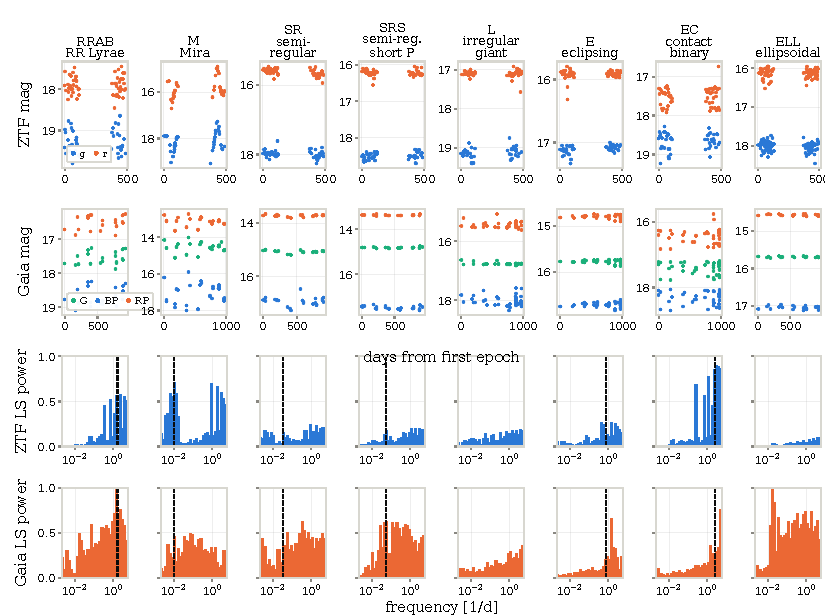
\includegraphics[width=\textwidth]{fig0_data_k4featdft_prod8.pdf}
  \caption{\textbf{The data, and what the model reconstructs.}
  One clear member of each VSX class, in ZTF $g$/$r$ (\emph{row 1}) and the same star in Gaia $G$/$BP$/$RP$ (\emph{row 2}); columns run from clean-period pulsators through the red-giant irregulars to the eclipsing binaries.
  \emph{Rows 3--4:} the 32-bin unfolded Schuster periodogram of each, the spectral half of the featurisation.
  The two surveys see the same physics through different cadences, depths and passbands, and the periodogram inherits the window function of each --- the confound the model is built to separate.
  The dashed line is the VSX period, which nothing downstream sees.}
  \label{fig:data}
\end{figure}

\paragraph{Model architecture.}
The model is a conditional flow-matching decoder over the 39 tokens, FiLM-conditioned on the concatenated latents of a physics encoder and an instrument encoder.
During training, an anchor view of object $n$ in survey $s$ is the flow-matching target and is never encoded.
The physics encoder sees the same object $n$ in the other survey $s'$; the instrument encoder sees $K=4$ different objects in the anchor's survey $s$, pooled by attention with a query built from the anchor's observing log.
The anchor survey alternates per sample, which is what forces the physics encoder to be instrument-invariant: it can only succeed by extracting what survives a change of instrument.
Both encoders are diagonal state-space models over the token axis, each compressing to a 4-dimensional latent, and the decoder receives, besides the latents, only the anchor's token coordinates and its two observing-log scalars --- never its level, amplitude or error.
No labels enter the loss; classes and catalogue parameters appear only in probes on the frozen latent.

\section{Results}

% ---------------------------------------------------------------- figure 2
\begin{figure}[t]
  \centering
  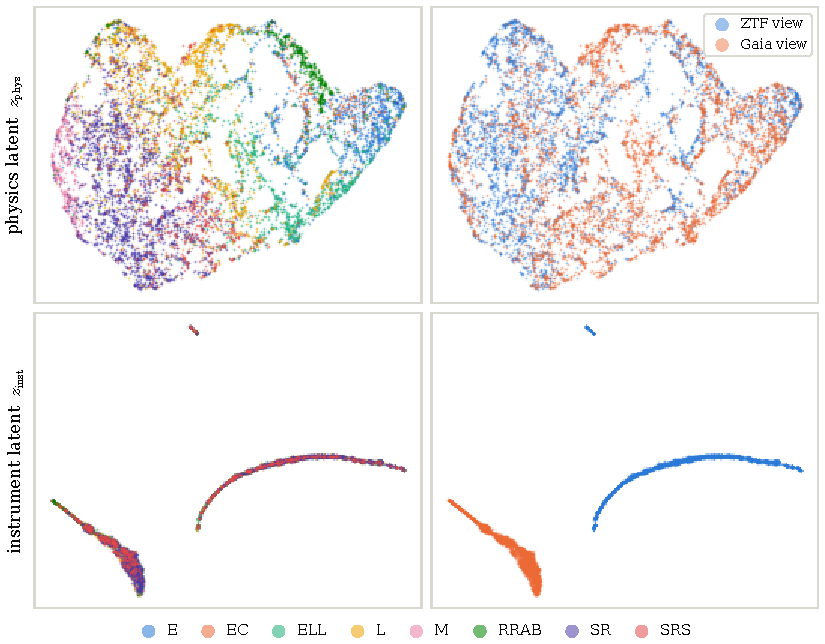
\includegraphics[width=\textwidth]{fig1_umap_roles_k4featdft_prod8.pdf}
  \caption{\textbf{The physics and instrument latent spaces, with both surveys embedded.}
  Each encoder's 4-dimensional space holds the ZTF and the Gaia view of every held-out star.
  \emph{Top:} the physics latent, coloured by VSX class and by survey.
  \emph{Bottom:} the instrument latent, coloured the same way.
  The physics latent organises the stars by class while the two surveys interweave; the instrument latent separates the surveys completely ($0.36$ against $0.00$ cross-survey neighbour overlap) and orders each by its observing log, with little class structure.}
  \label{fig:umap}
\end{figure}

% ---------------------------------------------------------------- figure 3
\begin{figure}[t]
  \centering
  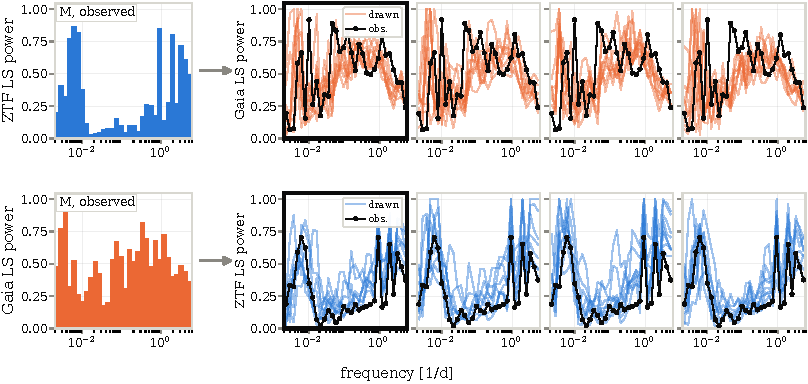
\includegraphics[width=\textwidth]{fig3_swap_recon_k4featdft_prod8.pdf}
  \caption{\textbf{Reconstruction and transfer, in both directions, on held-out objects.}
  \emph{Left:} the observed source periodogram, the view the physics encoder $\zphys$ sees.
  \emph{Right, across the arrow:} the same star drawn in the other survey, one panel per instrument conditioning $\zinst$, every flow sample as its own line and the observed destination periodogram in black.
  The heavy frame marks the base case, where the instrument role is the paired observation; the other panels fill it with strangers, so nothing about this star's destination view enters the model.
  The decoder draws the level, amplitude and error tokens as well; the periodogram is shown because it is where the transfer is legible.
  Objects sit near the median anomaly score of their class.}
  \label{fig:swap}
\end{figure}

% ------------------------------------------------- figure 4
\begin{figure}[t]
  \centering
  \begin{subfigure}{0.485\textwidth}
    \centering
    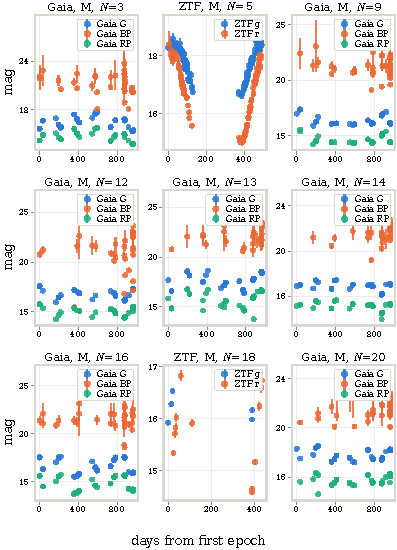
\includegraphics[width=\textwidth]{fig2_outliers_phys_k4featdft_prod8.pdf}
    \caption{\textbf{Physics latent.} Miras are enriched $4.8\times$ in this latent's top percentile, and it flags both survey views of the same star for $3.0\%$ of it, ten times the instrument latent's rate.
    Panels are the nine highest-ranked Miras, with $N$ each view's rank in the unrestricted ordering.}
    \label{fig:out_phys}
  \end{subfigure}
  \hfill
  \begin{subfigure}{0.485\textwidth}
    \centering
    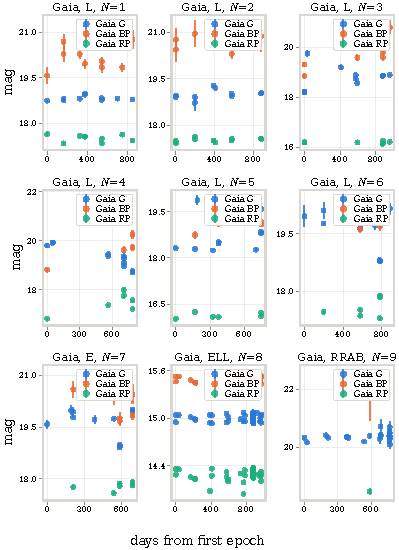
\includegraphics[width=\textwidth]{fig2_outliers_inst_k4featdft_prod8.pdf}
    \caption{\textbf{Instrument latent.} The top percentile is $92\%$ Gaia views, and the leading panels are sparse ones --- twenty to thirty rows against a median of eighty-three --- with no Mira enrichment.
    It flags views, not stars.}
    \label{fig:out_inst}
  \end{subfigure}
  \caption{\textbf{What each latent calls an outlier.}
  The nine strongest $k$-NN outliers of each latent, ranked over both surveys at once.
  Each panel names the survey the flagged view comes from, its class and $N$, its rank in that latent's ordering.
  Neither latent was given labels, epoch counts or cadence in training.}
  \label{fig:outliers}
\end{figure}

% ---------------------------------------------------------------- figure 5
\begin{figure}[t]
  \centering
  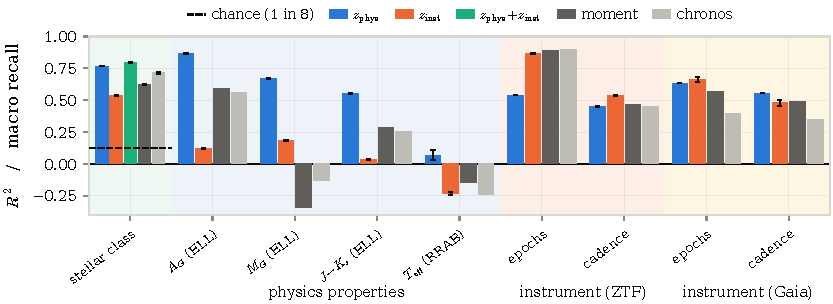
\includegraphics[width=\textwidth]{fig4_probe_r2_k4featdft_prod8.pdf}
  \caption{\textbf{Our two latents against two pretrained foundation models.}
  Each bar is a frozen representation scored on the same held-out split by the same probe.
  The stellar-class bars are macro recall over eight VSX classes, averaged over four probe seeds, with the concatenated latent added; every other bar is a magnitude-controlled $R^2$.
  The combined 8-dimensional latent classifies better than either foundation embedding, and the physics latent alone leads every stellar parameter shown; the period is the one target it does not lead, and is discussed in the text.
  On the instrument side the instrument latent leads its own survey's observing log while the physics latent leads Gaia's, which is the confound the magnitude control polices.
  The physics and instrument latents dissociate --- the physics bars belong to one and the ZTF observing-log bars to the other --- which is what licenses the anomaly readings of Fig.~\ref{fig:outliers}.}
  \label{fig:probes}
\end{figure}

\section{Discussion}
The Mira period is the one continuous target where the foundation models lead, and it is not a failure of the input: the 39 frozen tokens recover the period at $R^2\approx0.8$, matching the foundation models, and a four-dimensional linear projection of those tokens keeps almost all of it.
The loss is in the objective. Reconstruction draws place the periodogram's peak in the correct bin in roughly one draw in ten for ZTF anchors and one in six for Gaia, above chance but far from placed: a flow matched on every token equally pays for level and colour, which shape all 39 tokens, and not for a peak that occupies two of them, so the encoder is under no pressure to carry it.
The level and colour tokens, which the same objective does pay for, are where the physics latent leads.
Paying the objective for the peak, or giving the peak its own token to reconstruct, is the next experiment.

Gaia's photometric error is photon-limited, so once median magnitude is
controlled the residual tracks variability amplitude rather than the
instrument, which is why $\zphys$ leads that bar while $\zinst$ leads its ZTF
counterpart.

\section*{References}
{\small
TODO.
}

\appendix
\section{Encoder ablation}
% ---------------------------------------------------------------- table 1
% Generated by compare_encoders.py --latex; regenerate rather than hand-edit.
MIGHT KILL TABLE, METRIC UNCLEAR

\begin{table}[h]
  \centering
  \footnotesize
  \begin{tabular}{l r r r r r r r r r}
\toprule
& & & \multicolumn{2}{c}{val loss $\downarrow$} & & \multicolumn{2}{c}{class, $\zphys$ $\uparrow$} & & \\
\cmidrule(lr){4-5}\cmidrule(lr){7-8}
Encoder & Par. & s/ep & ZTF & Gaia & RMSE $\downarrow$ & ZTF & Gaia & $\zinst$ $\uparrow$ & align $\uparrow$ \\
\midrule
S4D & 398.5k & 16 & 0.1397 & 0.1975 & 0.348 & 0.471 & 0.541 & 0.211 & 0.71 \\
Conformer & 392.9k & 22 & 0.1395 & 0.1961 & 0.352 & 0.472 & 0.562 & 0.186 & 0.17 \\
GRU & 401.3k & 60 & 0.1395 & 0.2015 & 0.325 & 0.489 & 0.562 & 0.175 & 0.48 \\
Dilated conv & 399.4k & 13 & 0.1408 & 0.1973 & 0.347 & 0.413 & 0.547 & 0.177 & 0.18 \\
\bottomrule
\end{tabular}

  \caption{\textbf{Swapping the encoder's sequence mixer barely moves the
  representation.}
  Four sequence models --- a diagonal state space, a convolution-augmented
  transformer, a bidirectional GRU and a dilated convolution --- are each sized
  to the same encoder parameter count and swapped in behind an otherwise
  identical model.
  They land in a narrow band on validation loss, and the ranking is not
  consistent between the loss, the reconstruction and the probes.
  Cost is not so flat: the recurrent encoder spends roughly four times the step
  time of the convolutional one for nothing the probes can resolve.
  Two columns do separate them --- the strictly local convolution is the
  weakest at classifying the sparser ZTF view, and the state space model is
  alone in aligning a star's two survey views, which is the property the design
  exists to produce.
  Validation loss is split by anchor direction rather than pooled, because
  Gaia's photometry is the more precise of the two and a pooled figure can hide
  one direction degrading as the other improves.
  \emph{align} is the cosine alignment of a star's two survey views under
  $\zphys$, minus its own shuffled baseline; the class columns are linear
  probes on the frozen latent, macro over eight classes.
  One seed throughout, so differences below $\sim$0.01 sit inside the spread of
  a single run.}
  \label{tab:encoders}
\end{table}


\end{document}
